En esta sección presentamos las herramientas utilizadas para este trabajo. Así también como los comandos con los que se realizó en preentrenamiento, el entrenamiento y la generación de oraciones para la tesis.

\subsection{Festival y Festvox: Generación las transcripciones fonéticas}

Festival es un framework que permite sintetizar habla. Además posee una gran variedad de APIs, para el procesamiento de audios y generación de nuevos sistemas TTS. Festvox a su vez expande sobre Festival, agregando todavía más herramientas relacionadas a la síntesis y generación de modelos, que van desde la generación de modelos prosódicos, hasta etiquetado automático de corpus.

Para este trabajo utilizaremos Festival y Festvox para generar los oraciones requeridos tanto para el entrenamiento como para la síntesis de audios. Estos consisten básicamente en una transcripción fonética de los audios dividida en segmentos temporales y datos contextuales tales como la cantidad de silabas en la palabra siendo transcrita, fonemas que preceden y proceden al actual, etc.

A modo de guía a continuación mostraremos como es que utilizamos estas herramientas para generar las transcripciones fonéticas deseadas usando EHMM alignment.

Primero tendremos que generar un archivo \textit{txt.done.data} donde estén los nombres de cada archivo de audio y su transcripción grafemica. Por ejemplo, en el siguiente recuadro podemos ver un extracto del archivo generado para SECYT\_mm utilizado para este proceso:

\begin{tcolorbox}
( SECYT\_mm\_1\_335 ``Algunos dicen gamba en vez de pierna'' )

( SECYT\_mm\_1\_29 ``El conjunto de las escenas se reitera en el galpón'' )

( SECYT\_mm\_1\_361 ``Lluvia con truenos en Medellín'' )

( SECYT\_mm\_1\_619 ``Rendían pleistecía vikingo conquistador'' )

( SECYT\_mm\_1\_110 ``Llueve sobre las piedras de la pared'' )

( SECYT\_mm\_1\_102 ``Las etapas del desarrollo infantil difieren según el niño'' )

\end{tcolorbox}

En este trabajo utilizamos Festival $2.4$\cite{festivalDownload}, Festvox $2.7$\cite{festvoxDownload} y speech\_tools $2.4$\cite{speechToolDownload} para la generación de transcripciones fonéticas. Para poder utilizarlos agregamos las siguientes variables de entorno en nuestro PATH:

\begin{tcolorbox}
export PATH=/project/festival/bin:\$PATH

export PATH=/project/speech\_tools/bin:\$PATH

export FESTVOXDIR=/project/festvox

export ESTDIR=/project/speech\_tools
\end{tcolorbox}

Luego generamos los directorios, scripts y archivos necesarios para generar una nueva voz:
%referencia
%https://github.com/zeehio/festvox/blob/master/src/clustergen/setup_cg
\begin{tcolorbox}
\$FESTVOXDIR/src/clustergen/setup\_cg uba es SECYT\_mm
\end{tcolorbox}

En la nueva estructura de archivos generada, copiar los audios en la carpeta wav/ y el archivo \textit{txt.done.data} previamente generado en la carpeta etc/.

Además en los archivos 

\begin{tcolorbox}
festvox/uba\_es\_\_cg.scm 

festvox/uba\_es\_\_clunits.scm
\end{tcolorbox}

Es necesario cambiar las dependencias 

\begin{tcolorbox}
(require 'uba\_es\_\_phoneset)

(require 'uba\_es\_\_lexicon)
\end{tcolorbox}

que contienen los simbolos fonéticos del español de España, por estas otras

\begin{tcolorbox}
(require 'uba\_es\_\_phoneset\_mex)

(require 'uba\_es\_\_lexicon\_mex)
\end{tcolorbox}

que contienen el conjunto de símbolos fonéticos del español mexicano que se aproximan de manera muy cercana a los del castellano río platense (no contiene /th/ por ejemplo).

Finalmente corriendo los siguientes comandos:

\begin{tcolorbox}
./bin/do\_build build\_prompts

./bin/do\_build label

./bin/do\_build build\_utts
\end{tcolorbox}

Se realizará el proceso de alineamiento y transcripción automática. Una vez finalizado se habrán generado las transcripciones fonéticas con formato .utt en el directorio festival/utts, que entre otra metadata tiene codificados los fonos de la oración, sus principios y sus finales.

De manera análoga, esta herramienta te permite crear transcripciones fonéticas para la síntesis. Simplemente generando un archivo \textit{txt.done.data} con oraciones que se quieran sintetizar, y corriendo el script

\begin{tcolorbox}
./bin/do\_build build\_prompts ./synth/txt.done.data
\end{tcolorbox}

En la carpeta utt gen/prompt-utt se habrán generado los .utt necesarios para la síntesis.


\subsection{HTS}


HTS es un framework de entrenamiento y síntesis de sistemas TTS basado en HMMs que modela simultáneamente la duración, el espectro (mel-cepstrum) y la frecuencia principal ($f0$) de utilizando una combinación de HMMs:

\begin{figure}
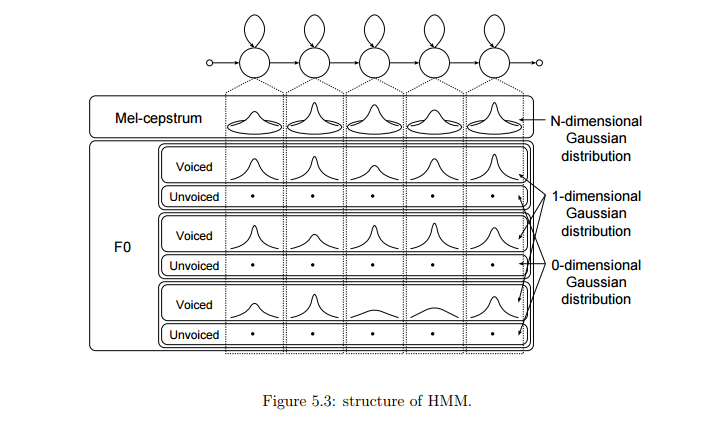
\includegraphics[scale=0.5]{imagenes/hmm.png}
\caption{Estructura de un hmm (simultaneous modeling of phonetic and prosodic parameters, and characteristic conversion for hmm-based text-to-speech systems, takayoshi yoshimura, january 2002, pag. 41)}
\label{hmmStructure}
\centering
\end{figure}

Como se ve en la figura \ref{hmmStructure} el espectro y la frecuencia fundamental son modelados en paralelo usando vectores separados. En particular el espectro será modelado como un vector de gaussianas $n$ dimensional, mientras que la frecuencia principal será modelado como conjunto de vectores de gaussianas de dimensión uno y cero.

Al mismo tiempo HTS toma la decisión de modelar la información prosódica dentro de este mismo framework. Para esto, las distribuciones para el espectro, la frecuencia principal y las duraciones son clusterizadas independientemente utilizando la información contextual extraída de los audios de entrenamiento. A modo ilustrativo en la figura \ref{hmmTree} se muestra una esquematización de un HMM resultante utilizando arboles de decisión para clusterizar los datos. Notar que cada hoja del árbol resultante coincidirá con un vector $n$ dimensional de gaussianas o un conjunto de vectores de gaussianas de dimensión cero y uno, según corresponda al espectro o a la frecuencia principal.

\begin{figure}
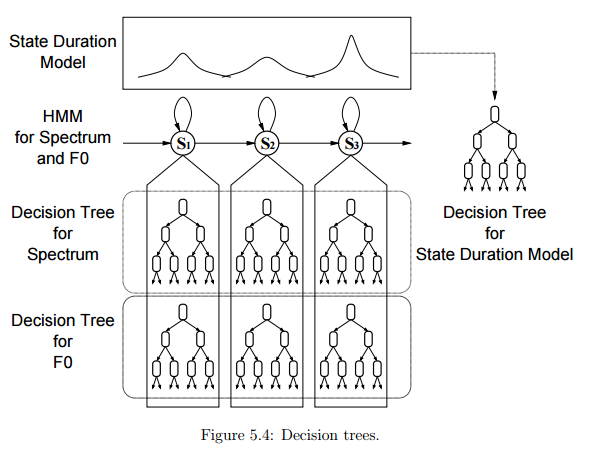
\includegraphics[scale=0.5]{imagenes/hmmContext.png}
\caption{Esquema HMM generado utilizando arboles de decisión (simultaneous modeling of phonetic and prosodic parameters, and characteristic conversion for hmm-based text-to-speech systems, takayoshi yoshimura, january 2002, pag. 45)}
\label{hmmTree}
\centering
\end{figure}
%hablar de los distintos tipos de clusters?

Si bien existen muchas maneras de clusterizar el conjunto de fonemas, que pueden variar desde algoritmos simples hasta técnicas de redes neuronales, para este trabajo todos los entrenamientos y clusterizaciones de datos se realizarán con arboles de decisión. 

Por otro lado como información contextual para el entrenamiento se tomaron los dos fonemas precedentes y los dos fonemas procedentes para cada fonema y la siguiente información fonética.

\begin{itemize}
\item Modo de articulación del fonema.
\item Punto de articulación del fonema.
\item La perspectiva articulatoria (anterior, central o posterior).
\item Si el fonema es una vocal o una consonante.
\item En caso de ser una vocal, a que categoría pertenece: por ejemplo para el fonema $/i/:$ {$i$ (no acentuada), $i0$ (diptongo) ,$i1$ (acentuada)}.
\item En caso de ser una vocal, su redondeamiento vocálico.
\item En caso de ser una consonante, si es lennis o fortis.
\end{itemize}

De esta manera HTS espera tener una voz mas dinámica, que para diferentes valores contextuales darán diferentes modelos acústicos para cada fonema.

En la imagen \ref{genTree} se muestra el resultado de un fragmento de uno de los arboles de decisión generado para modelar la duración de un fonema. En base a este modelo, el sistema podrá inferir por ejemplo que si el fonema actual no es nasal (C-Nasal) seguido de un stop (R-Stop), que no es el fonema $l$ estará modelado por función de probabilidad gaussiana definida en $dur\_s2\_7$.

\begin{figure}
\begin{center}
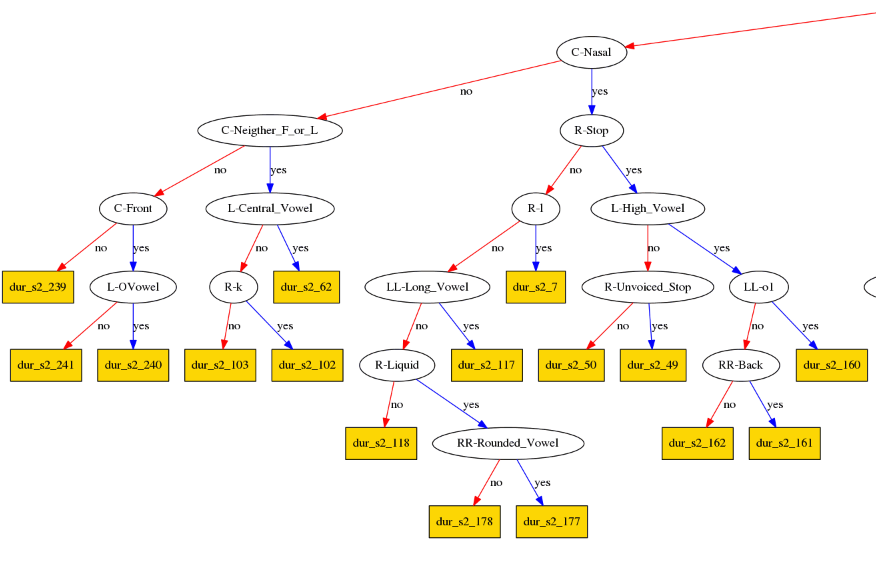
\includegraphics[scale=0.4]{imagenes/arbolDeDesicionTesis.png}
\caption{Árbol de decisión generado a partir de los datos para la duración de un HMM}
\label{genTree}
\end{center}
\end{figure}

En las primeras iteraciones del desarrollo no contábamos con la información acústica por lo que se generaron modelos carentes de información contextual. En estos primeros modelos se pudo apreciar una calidad mucho peor en los audios generados, sonando estos sumamente metálicos y carentes de prosodia. Esto se debía, posiblemente, a que los arboles de decisión no tenían información contextual suficiente para ser construidos de manera efectiva, resultando en una mala generalización y malos audios sintetizados. Tras agregar los factores contextuales y realizar algunas pruebas de concepto con ellas pudimos comprobar que las voces sonaban mucho mas humanas.


\subsection{Entrenamiento} \label{entrenamientoHTS}

Desde un punto de vista puramente tecnico, utilizar HTS para entrenar un modelo es bastante sencillo.

Asumiendo que todos los paquetes necesarios fueron instalados, es posible entrenar una nueva voz adaptando la demo disponible en la pagina de descargas de HTS.

Para ello, reemplazar los audios en la carpeta data/raw con aquellos aquellos que se quieran utilizar y los utts correspondientes previamente generados. 

Además como adelantamos en la sección anterior, será necesario indicarle a HTS que información contextual se utilizará para la clusterización, por lo que es necesario modificar el archivo data/questions/questions\_qst001.hed con la información contextual apropiada para una voz en castellano. En el apéndice \ref{apendiceQuestions} se presenta el archivo utilizado para Loc1\_pal.

Una vez finalizadas estas modificaciones, en la carpeta data/ de la demo puede iniciarse el pre entrenamiento de la siguiente manera:

\begin{tcolorbox}
make
\end{tcolorbox}

Que extraerá features del audio y construirá los archivos de entrenamiento a partir de los mismos entre otras cosas.

Finalmente para dar comienzo al entrenamiento, ejecutar en la carpeta raíz.

\begin{tcolorbox}
perl scripts/Training.pl scripts/Config.pm > train.log 2> err.log
\end{tcolorbox}

Una vez que se complete el entrenamiento, será posible encontrar en la carpeta X el modelo generado (.htsvoice).

Para este trabajo todos los audios usarán sampling rate de $48$kHz, precisión de $16$bits, mono. 

Además HTS nos pide que explicitemos un rango de extracción para frecuencia fundamental. Tanto para SECYT como para Loc1-Pal el rango utilizado fue desde $100$hz hasta $350$hz, mientras que para CMU-ARCTIC el rango de extracción fue desde $110$kHz hasta $280$kHz.

Estos parámetros y muchos otros pueden ser configurados fácilmente corriendo

\begin{tcolorbox}
./configure
\end{tcolorbox}

en la carpeta raíz del proyecto.

En la próxima sección detallaremos como utilizar varios .htsvoice generados para mezclar y sintetizar una nueva voz.

\subsection{HTS\_engine} \label{interpolationTeory}

Finalmente para generar voces con acento extranjero se utilizó hts\_engine. Esta herramienta permite interpolar con pesos arbitrarios entre varios modelos para producir un nuevo modelo con una mezcla de la carga fonética y prosódica de ambos hablantes y sintetizar audios. Esto nos brinda un gran rango exploratorio y nos permitirá ajustar la carga fonética de los modelos originales para acercarnos al modelo deseado. 

A grandes rasgos la interpolación consistirá en tomar los vectores generados anteriormente durante el entrenamiento e interpolar sus funciones de densidad gaussianas para obtener una nueva. En la imagen \ref{spekerInterpolationImagen} (extraída del trabajo \cite{SpekerInterpolationRef}) puede verse la interpolación de $N$ HMMs, cada uno con peso arbitrario $a_1$, $a_2$, ..., $a_N$, que generaran un nuevo modelo $\Lambda$.

\begin{figure}
\begin{center}
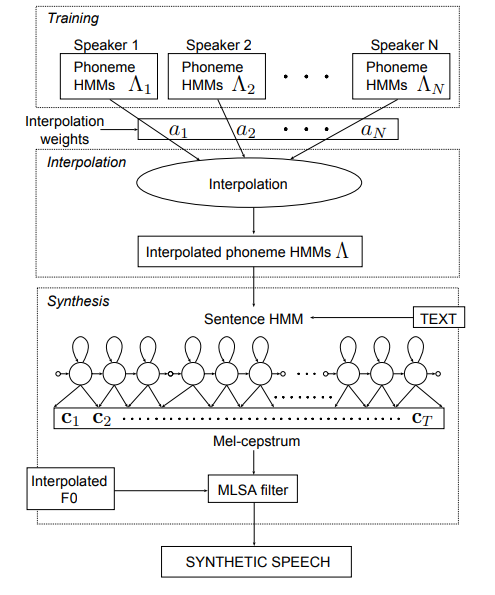
\includegraphics[scale=0.4]{imagenes/speakerInterpolation.png}
\caption{Block diagram of speech synthesis system with speaker interpolaiton. }
\label{spekerInterpolationImagen}
\end{center}
\end{figure}

Una vez obtenido el nuevo HMM es generado el proceso de síntesis puede ocurrir como para cualquier otro modelo, ilustrado en la etapa de síntesis de la figura.

El proceso de síntesis es bastante simple. Asumiendo que todos todas las dependencias fueron instaladas de manera correcta, con el siguiente comando, es posible utilizar los modelos generados en \textit{cmu\_us\_arctic\_slt.htsvoice} y \textit{models/loc1\_pal.htsvoice} para interpolar con peso $0.7$ y $0.3$ respectivamente, generar un nuevo modelo y sintetizar la oración presente en el archivo in.lab.

\begin{tcolorbox}
hts\_engine -m models/cmu\_us\_arctic\_slt.htsvoice -m models/loc1\_pal.htsvoice -i 2 0.7 0.3 -ow out.wav in.lab
\end{tcolorbox}

Esta herramienta permite además modificar el pitch, duración del audio y otros aspectos de la síntesis. La documentación completa puede encontrarse en http://hts-engine.sourceforge.net/.